%%%%%%%%%%%%%%%%%%%%%%%%%%%%%%%%%%%%%%%%%
% Compact Laboratory Book
% LaTeX Template
% Version 1.0 (4/6/12)
%
% This template has been downloaded from:
% http://www.LaTeXTemplates.com
%
% Original author:
% Joan Queralt Gil (http://phobos.xtec.cat/jqueralt) using the labbook class by
% Frank Kuster (http://www.ctan.org/tex-archive/macros/latex/contrib/labbook/)
%
% License:
% CC BY-NC-SA 3.0 (http://creativecommons.org/licenses/by-nc-sa/3.0/)
%
% Important note:
% This template requires the labbook.cls file to be in the same directory as the
% .tex file. The labbook.cls file provides the necessary structure to create the
% lab book.
%
% The \lipsum[#] commands throughout this template generate dummy text
% to fill the template out. These commands should all be removed when 
% writing lab book content.
%
% HOW TO USE THIS TEMPLATE 
% Each day in the lab consists of three main things:
%
% 1. LABDAY: The first thing to put is the \labday{} command with a date in 
% curly brackets, this will make a new section showing that you are working
% on a new day.
%
% 2. EXPERIMENT/SUBEXPERIMENT: Next you need to specify what 
% experiment(s) and subexperiment(s) you are working on with a 
% \experiment{} and \subexperiment{} commands with the experiment 
% shorthand in the curly brackets. The experiment shorthand is defined in the 
% 'DEFINITION OF EXPERIMENTS' section below, this means you can 
% say \experiment{pcr} and the actual text written to the PDF will be what 
% you set the 'pcr' experiment to be. If the experiment is a one off, you can 
% just write it in the bracket without creating a shorthand. Note: if you don't 
% want to have an experiment, just leave this out and it won't be printed.
%
% 3. CONTENT: Following the experiment is the content, i.e. what progress 
% you made on the experiment that day.
%
%%%%%%%%%%%%%%%%%%%%%%%%%%%%%%%%%%%%%%%%%

%----------------------------------------------------------------------------------------
%	PACKAGES AND OTHER DOCUMENT CONFIGURATIONS
%----------------------------------------------------------------------------------------                               

\documentclass[fontsize=11pt, % Document font size
                             paper=a4, % Document paper type
                             twoside, % Shifts odd pages to the left for easier reading when printed, can be changed to oneside
                             captions=tableheading,
                             index=totoc,
                             hyperref]{labbook}
 
\usepackage[bottom=10em]{geometry} % Reduces the whitespace at the bottom of the page so more text can fit

\usepackage[english]{babel} % English language
\usepackage{lipsum} % Used for inserting dummy 'Lorem ipsum' text into the template

\usepackage[utf8]{inputenc} % Uses the utf8 input encoding
\usepackage[T1]{fontenc} % Use 8-bit encoding that has 256 glyphs

\usepackage[osf]{mathpazo} % Palatino as the main font
\linespread{1.05}\selectfont % Palatino needs some extra spacing, here 5% extra
\usepackage[scaled=.88]{beramono} % Bera-Monospace
%\usepackage[scaled=.86]{berasans} % Bera Sans-Serif
\usepackage[rm,light]{roboto} % Roboto

\usepackage{booktabs,array} % Packages for tables

\usepackage{amsmath} % For typesetting math
\usepackage{graphicx} % Required for including images
\usepackage{etoolbox}
\usepackage[norule]{footmisc} % Removes the horizontal rule from footnotes
\usepackage{lastpage} % Counts the number of pages of the document

\usepackage[dvipsnames]{xcolor}  % Allows the definition of hex colors
\definecolor{titleblue}{rgb}{0.16,0.24,0.64} % Custom color for the title on the title page
\definecolor{linkcolor}{rgb}{0,0,0.42} % Custom color for links - dark blue at the moment

\addtokomafont{title}{\Huge\color{titleblue}} % Titles in custom blue color
\addtokomafont{chapter}{\color{OliveGreen}} % Lab dates in olive green
\addtokomafont{section}{\color{Sepia}} % Sections in sepia
\addtokomafont{pagehead}{\normalfont\sffamily\color{gray}} % Header text in gray and sans serif
\addtokomafont{caption}{\footnotesize\itshape} % Small italic font size for captions
\addtokomafont{captionlabel}{\upshape\bfseries} % Bold for caption labels
\addtokomafont{descriptionlabel}{\rmfamily}
\setcapwidth[r]{10cm} % Right align caption text
\setkomafont{footnote}{\sffamily} % Footnotes in sans serif

\deffootnote[4cm]{4cm}{1em}{\textsuperscript{\thefootnotemark}} % Indent footnotes to line up with text

\DeclareFixedFont{\textcap}{T1}{phv}{bx}{n}{1.5cm} % Font for main title: Helvetica 1.5 cm
\DeclareFixedFont{\textaut}{T1}{phv}{bx}{n}{0.8cm} % Font for author name: Helvetica 0.8 cm

\usepackage[nouppercase,headsepline]{scrpage2} % Provides headers and footers configuration
\pagestyle{scrheadings} % Print the headers and footers on all pages
\clearscrheadfoot % Clean old definitions if they exist

\automark[chapter]{chapter}
\ohead{\headmark} % Prints outer header

\setlength{\headheight}{25pt} % Makes the header take up a bit of extra space for aesthetics
\setheadsepline{.4pt} % Creates a thin rule under the header
\addtokomafont{headsepline}{\color{lightgray}} % Colors the rule under the header light gray

\ofoot[\normalfont\normalcolor{\thepage\ |\  \pageref{LastPage}}]{\normalfont\normalcolor{\thepage\ |\  \pageref{LastPage}}} % Creates an outer footer of: "current page | total pages"

% These lines make it so each new lab day directly follows the previous one i.e. does not start on a new page - comment them out to separate lab days on new pages
\makeatletter
\patchcmd{\addchap}{\if@openright\cleardoublepage\else\clearpage\fi}{\par}{}{}
\makeatother
\renewcommand*{\chapterpagestyle}{scrheadings}

% These lines make it so every figure and equation in the document is numbered consecutively rather than restarting at 1 for each lab day - comment them out to remove this behavior
\usepackage{chngcntr}
\counterwithout{figure}{labday}
\counterwithout{equation}{labday}

% Hyperlink configuration
\usepackage[
    pdfauthor={}, % Your name for the author field in the PDF
    pdftitle={Laboratory Journal}, % PDF title
    pdfsubject={}, % PDF subject
    bookmarksopen=true,
    linktocpage=true,
    urlcolor=linkcolor, % Color of URLs
    citecolor=linkcolor, % Color of citations
    linkcolor=linkcolor, % Color of links to other pages/figures
    backref=page,
    pdfpagelabels=true,
    plainpages=false,
    colorlinks=true, % Turn off all coloring by changing this to false
    bookmarks=true,
    pdfview=FitB]{hyperref}

\usepackage[stretch=10]{microtype} % Slightly tweak font spacing for aesthetics

%\setlength\parindent{0pt} % Uncomment to remove all indentation from paragraphs

%----------------------------------------------------------------------------------------
%	DEFINITION OF EXPERIMENTS
%----------------------------------------------------------------------------------------

% Template: \newexperiment{<abbrev>}[<short form>]{<long form>}
% <abbrev> is the reference to use later in the .tex file in \experiment{}, the <short form> is only used in the table of contents and running title - it is optional, <long form> is what is printed in the lab book itself

\newexperiment{example}[Example experiment]{This is an example experiment}
\newexperiment{example2}[Example experiment 2]{This is another example experiment}
\newexperiment{example3}[Example experiment 3]{This is yet another example experiment}

\newsubexperiment{subexp_example}[Example sub-experiment]{This is an example sub-experiment}
\newsubexperiment{subexp_example2}[Example sub-experiment 2]{This is another example sub-experiment}
\newsubexperiment{subexp_example3}[Example sub-experiment 3]{This is yet another example sub-experiment}

%----------------------------------------------------------------------------------------

\begin{document}

%----------------------------------------------------------------------------------------
%	TITLE PAGE
%----------------------------------------------------------------------------------------

\title{\textcap{Salton Sea Modeling Journal \\[1cm]  
\textaut{Beginning Jan-08-2015}}}

\author{
    \textaut{Valerie Sahakian}\\ \\ % Your name
     % Your degree
}
\date{} % No date by default, add \today if you wish to include the publication date

\maketitle % Title page

\printindex
\tableofcontents % Table of contents
\newpage % Start lab look on a new page

\begin{addmargin}[4cm]{0cm} % Makes the text width much shorter for a compact look

\pagestyle{scrheadings} % Begin using headers

%----------------------------------------------------------------------------------------
%	LAB BOOK CONTENTS
%----------------------------------------------------------------------------------------

\labday{Thursday, 8 January 2015}



%-----------------------------------------

\experiment{Modeling varying interfaces for the SSAF}

Try various surface expressions of the high-velocity interface to investigate how well-constrained this is, and if the interface is more likely to be to the East or West of the SSAF surface trace.  This will aid in determining what fault structure is present; if the fault is to the west of the surface trace of the SSAF, it is more likely a normal fault in the Salton Sea, not visible on land.  If it intersects the surface trace, it is likely that the fault may have a westward dip/oblique component; if to the east, there may be a larger normal fault cross-cutting the modern-day SSAF.

To modify the starting model and adjust the interface's surface trace, use the script:

/Modeling/salton\_line7base/vm/line7tomographymodels\_

/salton7base\_manip2.m

\subexperiment{Last time...Inversions 11, 12, and 13}

In October, inversions 12 and 13 were run; it turns out the "final" model I had before did not include constraints on the interface from the MCS reflector picks.  Inversions 12, and the final (13) were to correct this.  

\begin{figure}[h!]
\raggedleft
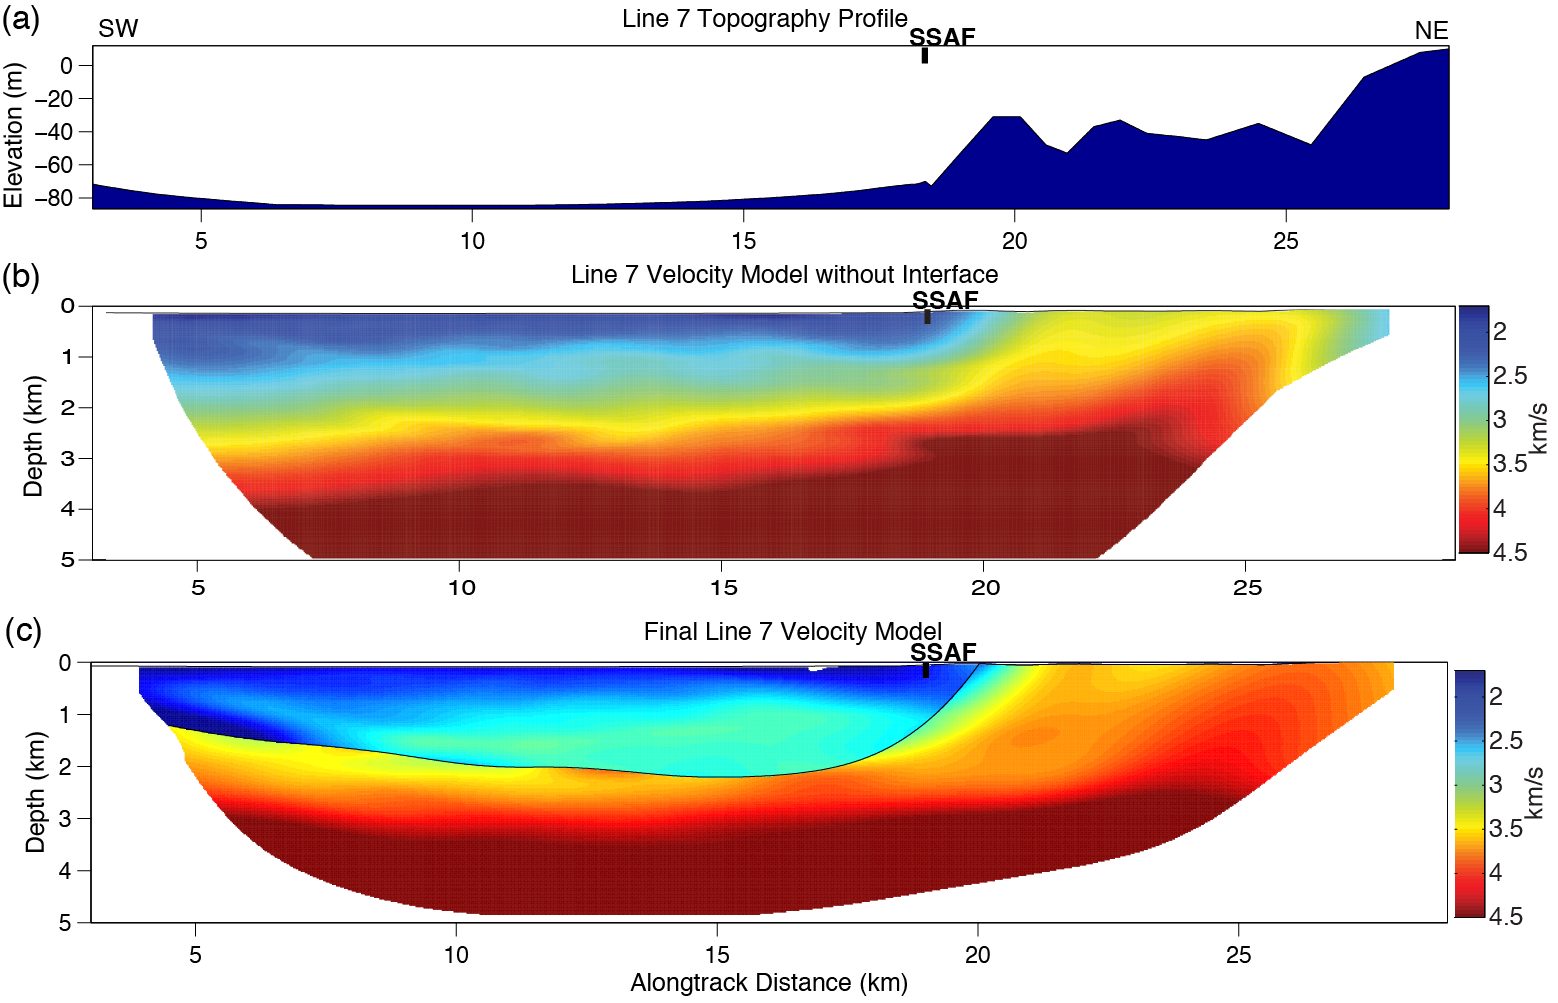
\includegraphics[scale=0.5,keepaspectratio=true]{figs/Salton7base_final11_topo_edit2.png}
\caption{Inversion 11 final model, without MCS constraints. (a) shows a topography profile; (b) shows the model without an interface; (c) shows the final model, with no MCS constraints, and with an interface.   Chi sq = 1.3.  }
\label{fig:line7noMCS}
\end{figure}

Inversions 12 and 13 were run with MCS constraints; the final model had a poorer chi sq than the other model; the question was why.  The best misfit came from inversion iteration 21, raytracing iteration 22, after applying the nullspace shuttles method.  This chi sq was 1.88, whereas without the MCS data it's 1.3.  The differences between the two are not that great, but with the MCS constraints the model looks a little splotchier because of where the layer 1 rays are turning.  The original final model, from inversion 11, can be seen in figure \autoref{fig:line7noMCS}; the final model with MCS constraints is seen in \autoref{fig:line7MCS}.  


\begin{figure}[h!]
\raggedleft
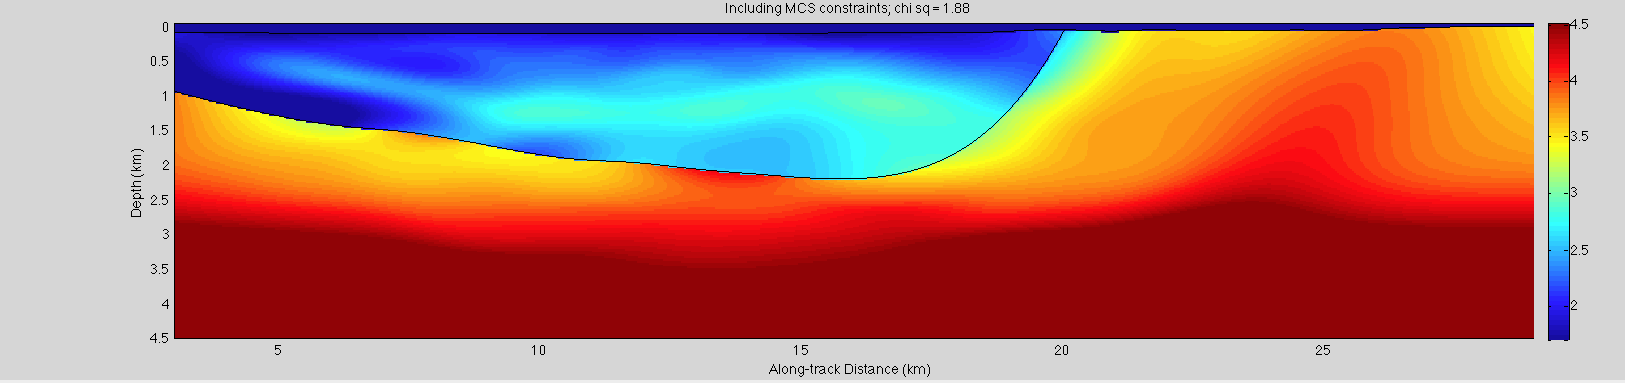
\includegraphics[scale=0.3,keepaspectratio=true]{figs/Line7_withMCS.png}
\caption{Inversion 13 final model, with MCS constraints.  Chi sq = 1.88.}
\label{fig:line7MCS}
\end{figure}

Alistair suggested looking at the reflection residuals:  

"I would look at how well, or not, the prediction of the previous model simply fits the trend in MCS reflection times, i.e. does it predict an increase in reflections times at about the same rate as seen in the MCS data?  If it does then it is possible that the is mostly a static time shift in your MCS picks relative to the OBS times.  If the trends aren't really compatible then you probably are doing about as well as you can in reconciling the different data within an single model.  and we should probably reconsider the possibility of the MCS reflections transgressing velocity contours."

To determine if this higher misfit is due to a consistently offset reflector, I plotted the just the reflection ray paths of the model with MCS constraints (\autoref{fig:line7MCS-resid}).   

\begin{figure}[h!]
\raggedleft
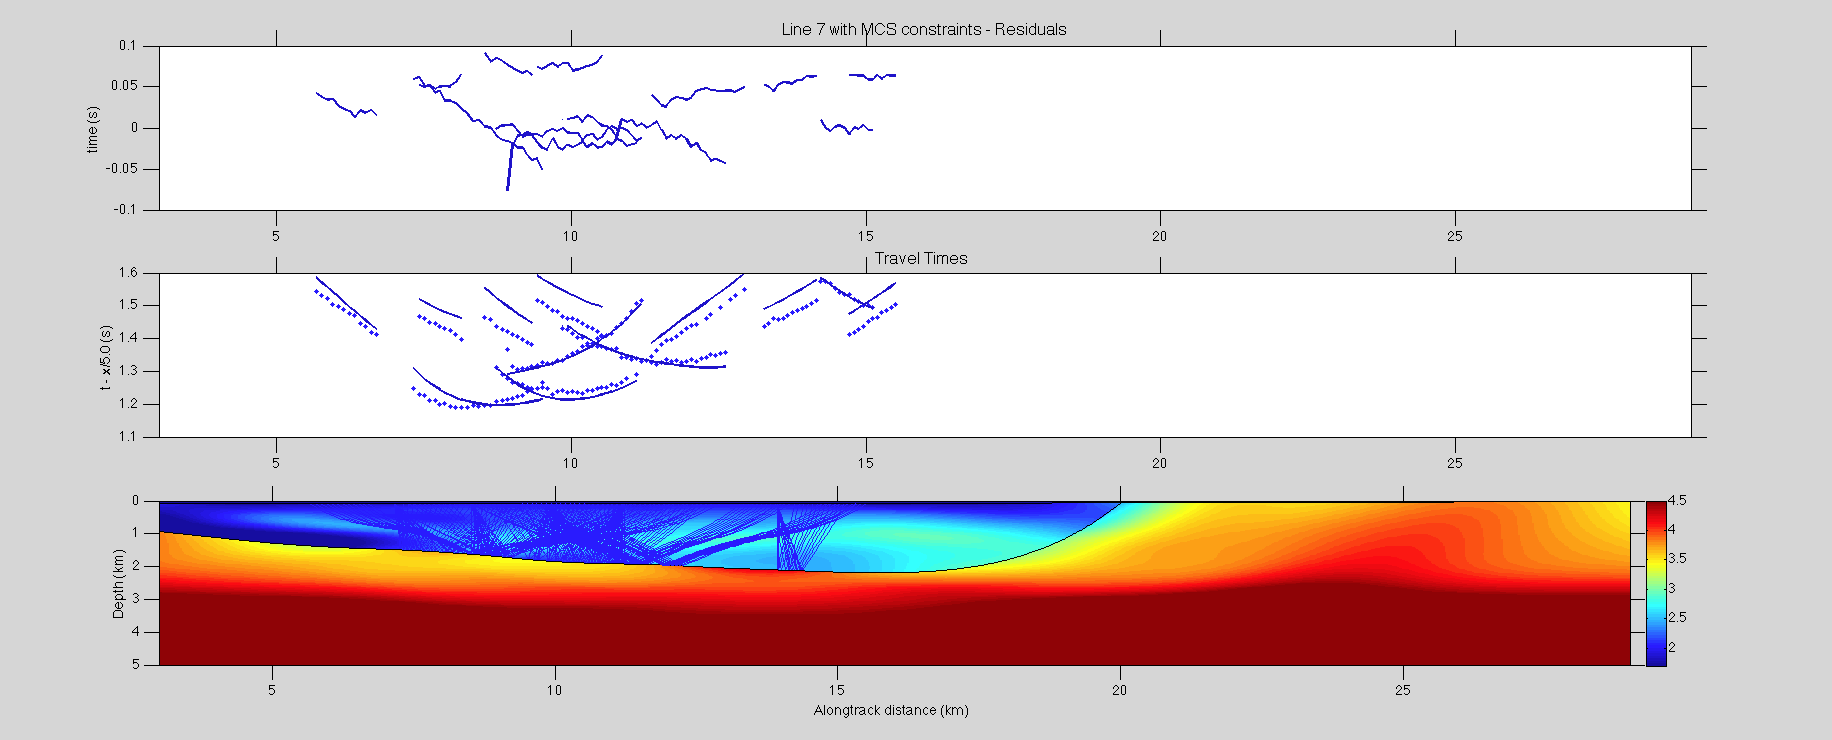
\includegraphics[scale=0.29,keepaspectratio=true]{figs/line7_resid_MCSconstraints.png}
\caption{Inversion 13 final model ray path residuals.}
\label{fig:line7MCS-resid}
\end{figure}


%Footnote example\footnote{Lorem ipsum dolor sit amet, consectetuer adipiscing elit.}.\\

%Citation example \cite{lamport94}.

%-----------------------------------------

\subexperiment{Inversion 14}

Start running inversions with varying interface surface traces.  For inversion 14, run an example with the SSAF trace set at x=18.94299186; this is commented in salton7base\_manip2.m.  

The starting model is under inversion14, and is named salton7base\_14\_0.vm, seen in \autoref{fig:startm14}.  This inversion will include constraints from MCS data; therefore, the file salton7base\_1\_4.ray will be included; this is the ray file for the MCS reflector picks.  The raytracing csh file is salton7base\_raytr14.csh and includes append = 1, so that the rays from the MCS file will be appended to the rayfan.  

The other settings are as follows:

set maxnode = 300,        
set cmax = 0.75,
set gdx = 1041,
set gdy = 1,
set gdz = 323

set stx = 10,
set sty = 0,
set stz = 9,
set ang = 0.5

set tstat = 0.0,
set xextension = 2.0,
set yextension = 2.0

Rayfan plotting is in script 
plot\_salton7\_raypaths\_14.m.

The inversion csh file is salton7base\_14.csh.  The parameters are as follows:

set sr = 10.0, set sz = 5.0

set slh =  0.02,
set jph =  0.005,
set rfh =  0.1,
set tstath = 0.04

set reg0 =    1.0, set reg1 =    1.0, set reg2 =   4.0

set asr = 5.0

set crf = 2, set cjp = 1

\begin{figure}[h!]
\raggedleft
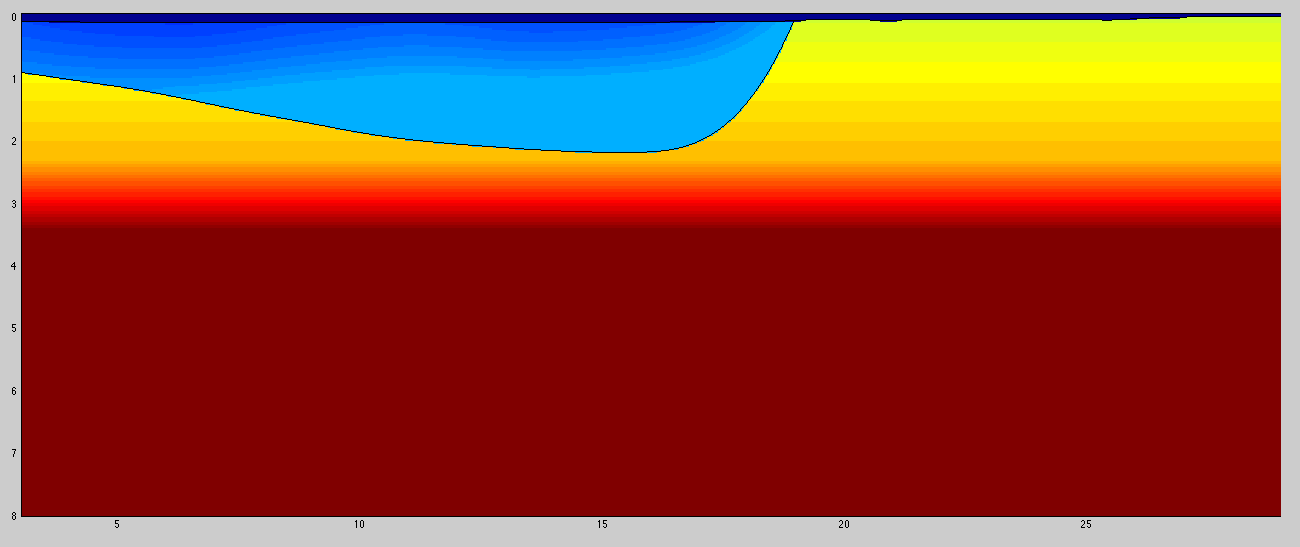
\includegraphics[scale=0.3,keepaspectratio=true]{figs/inv14_0.png}
\caption{Inversion 14 starting model.}
\label{fig:startm14}
\end{figure}







%-----------------------------------------

\subexperiment{Raytracing and Inversion Output}
Found in the tables \autoref{tab:r14}, \autoref{tab:i14}.
%\section{}
%Raytr it 
\begin{table}[ht]
\label{tab:r14}
\raggedleft
\begin{tabular}{c l l l l l}
\toprule
\textbf{Raytr, It = } & \textbf{tmean} & \textbf{trms} & \textbf{chi sq} & \textbf{chi r} & \textbf{meanErr} \\
\toprule
It0 & -0.0514 & 0.1174 & 73.2913 & 50.0788 & 0.0241\\
It1 & -0.0182 & 0.1075 & 47.3309 & 43.8783 & 0.0241\\
It2 & -0.0068 & 0.0906 & 25.6917 & 25.2468 & 0.0241\\
It3 & -0.0131 & 0.0644 & 14.3934 & 13.6786 & 0.0241\\
It4 & -0.0135 &  0.0527 & 8.7668 & 8.3057 & 0.0241\\
It5 & -0.0110 & 0.0446 & 5.2944 & 5.2898 & 0.0241\\
It6 & -0.0117 & 0.0382 & 3.1804 & 3.3014 & 0.0241\\
It7 & -0.0116 & 0.0360 & 2.5369 & 2.7169 & 0.0241\\
It8 & -0.0112 & 0.0349 & 2.2200 & 2.4544 & 0.0241\\
It9 & -0.0116 & 0.0339 & 2.0821 & 2.3345 & 0.0241\\
It10 & -0.0110 & 0.0338 & 1.9729 & 2.2349 & 0.0241\\
It11 & -0.0104 & 0.0336 & 1.9733 & 2.2920 & 0.0241\\
It12orig & -0.0108 & 0.0336 & 1.9329 & 2.2353 & 0.0241\\
It12 & -0.0039 & 0.0439 & 3.2228 & 3.4501 & 0.0241\\
It13 & -0.0114 & 0.0346 & 1.9718 & 2.1610 & 0.0241\\
It14 & -0.0112 & 0.0335 & 1.8335 & 2.1037 & 0.0241\\
It15 & -0.0101 & 0.0337 & 1.8931 & 2.2218 & 0.0241\\
It16 & -0.0120 & 0.0340 & 2.0673 & 2.2598 &  0.0241\\
\bottomrule\\
\end{tabular}
\caption{Inversion 14: Raytracing outputs.}
\end{table}

\clearpage

%INv it 
\begin{table}[ht]
\label{tab:i14}
\raggedleft
\begin{tabular}{c l l l}
\toprule
\textbf{Inv, It = } & \textbf{set chi sq =} & \textbf{out chi sq =} & \textbf{Penalty} \\
\toprule
It0 & 45 & 45.460 & 55886.17\\
It1 & 25 & 25.561 & 62766.52\\
It2 & 14 & 14.326 & 69724.12\\
It3 & 8 & 7.9459 & 75484.60\\
It4 & 5 & 4.9981 & 77469.94\\
It5 & 3 & 2.9994 & 86143.92\\
It6 & 2.3 & 2.3256 & 84903.17\\
It7 & 2.1 & 2.1429 & 81591.07\\
It8 & 1.8 & 1.8184 & 86594.72\\
It9 & 1.8 & 1.8618 & 83126.27\\
It10 & 1.8 & 1.8382 & 81169.54\\
It11 & 1.8 & 1.8382 & 79752.90\\
It12 & 2.0 & 2.0432 & 79529.48\\
It13 & 1.7 & 1.7128 & 83947.84\\
It14 & 1.7 & 1.7564 & 81046.24\\
It15 & 1.7 & 1.7376 & 79148.52\\
\bottomrule\\
\end{tabular}
\caption{Inversion 14: Inversion outputs.}
\end{table}

\clearpage

%----------------------------------------------------------------------------------------

\labday{Friday, 9 January 2015}
\experiment{Continuing Inversion 14}
Continuing from Thursday.  

\subexperiment{Inversion 14 steps and results}
Continued running Inversion 14 (output referenced in \autoref{tab:r14} and \autoref{tab:i14}).

Run nullspace shuttles on inversion iteration 11 (vm 12).  The pre-shuttled model, with a chi sq of 1.9329, is the best fit so far but is quite splotchy.  See in \autoref{fig:it11preshut}.  I used salton7\_shuttle\_update.m to create the shuttled model; 

\begin{figure}[h!]
\raggedleft
\includegraphics[scale=0.4,keepaspectratio=true]{../inversion14/figures/vm12_preshuttle.png}
\caption{Inversion 14, iteration 11 (vm 12), pre shuttle.}
\label{fig:it11preshut}
\end{figure}

Moving forwards, I named the output, shuttled model 

"Shuttles/line7shuttles/salton\_smshuttle\_inv14.vm".  This was copied into inversion14/, and renamed to salton7base\_14\_12.vm.
In inversion14, I renamed 12.ray, 12.vm, 12\_rough.vm, and 12\_raytr.out to orig.

In inversion\_temp, I renamed all iteration 11's to \_orig; including the anz, inz, nlr, rhsc, rhsn, sol, vecm\_in, and vecm\_out iteration 11's.  

\begin{figure}[h!]
\raggedleft
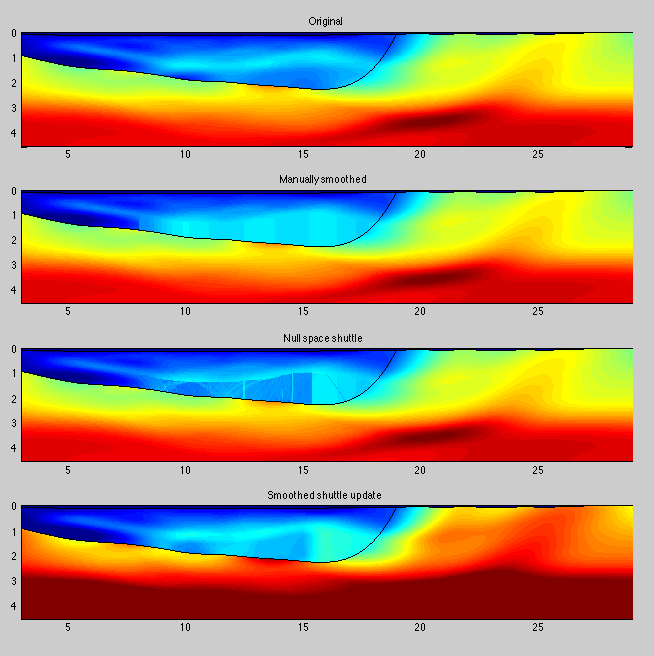
\includegraphics[scale=0.6,keepaspectratio=true]{figs/shuttlesInv14.png}
\caption{Inversion 14, iteration 11(vm12), post shuttle.}
\label{fig:it11postshut}
\end{figure}

After this, ray trace on the new shuttled model; so re-run raytracing iteration 12.  In the tables, the pre-shuttled statistics (raytracing it12) have been renamed to original.  The post-shuttled raytracing will be the new It12; this velocity model is in \autoref{fig:it11postshut}.

After several more iterations, I find that vm 14 (raytracing iteration 14, inversion iteration 13) has the lowest misfit (chi sq = 1.8335), and looks the "best" (the smoothest).  The final model is seen in \autoref{fig:inv14final}.  


\begin{figure}[h!]
\raggedleft
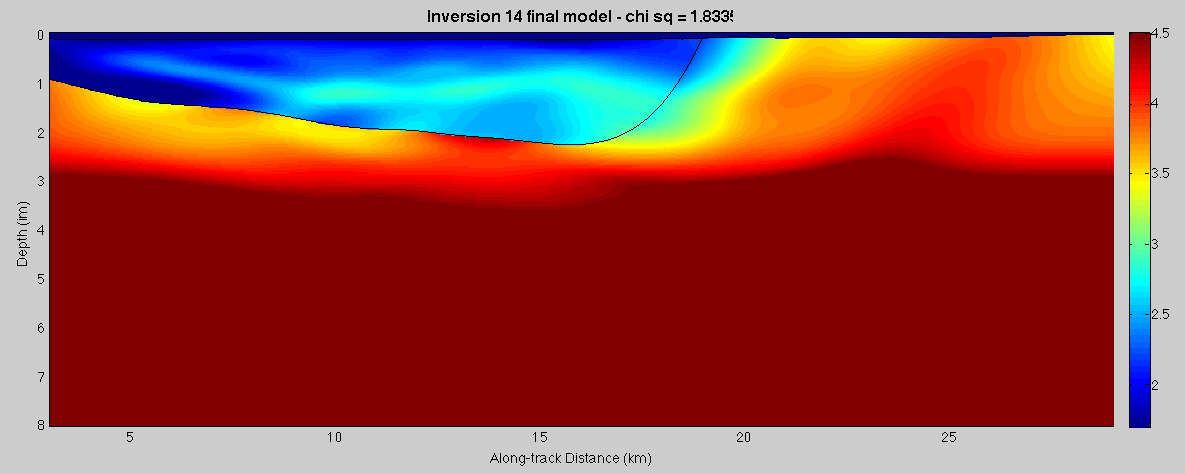
\includegraphics[scale=0.4,keepaspectratio=true]{figs/inv14_it13_FINAL.png}
\caption{Inversion 14, final model.  Vm number 14; chi sq = 1.8335.}
\label{fig:inv14final}
\end{figure}

\clearpage{}

%\experiment{example}
%
%\begin{equation}
%\label{eq:emc}
%e = mc^2
%\end{equation}
%
%Example equation citation: \autoref{eq:emc}.


%----------------------------------------------------------------------------------------
\labday{Thursday, 15 January 2015}

\experiment{Inversion 15 - Interface to the W of the SSAF trace}

Starting inversion 15.  Here, the interface intersects the surface at 17.9km along-profile, about 1 km west of the surface trace of the SSAF.  

To create the starting model, I once again used the script salton7base\_manip2.m.    The output model (starting model) is salton7base\_15\_0.vm, in inversion15/.  This is seen in \autoref{fig:inv15start}.  This inversion will include constraints from MCS data; therefore, the file salton7base\_1\_4.ray will be included; this is the ray file for the MCS reflector picks.  The raytracing csh file is salton7base\_raytr15.csh and includes append = 1, so that the rays from the MCS file will be appended to the rayfan.  

The other settings are as follows:

set maxnode = 300,        
set cmax = 0.75,
set gdx = 1041,
set gdy = 1,
set gdz = 323

set stx = 10,
set sty = 0,
set stz = 9,
set ang = 0.5

set tstat = 0.0,
set xextension = 2.0,
set yextension = 2.0


Rayfan plotting is in script 
plot\_salton7\_raypaths\_15.m.

The inversion csh file is salton7base\_15.csh.  The parameters are as follows:

set sr = 10.0, set sz = 5.0

set slh =  0.02,
set jph =  0.005,
set rfh =  0.1,
set tstath = 0.04

set reg0 =    1.0, set reg1 =    1.0, set reg2 =   4.0

set asr = 5.0

set crf = 2, set cjp = 1

\begin{figure}[h!]
\raggedleft
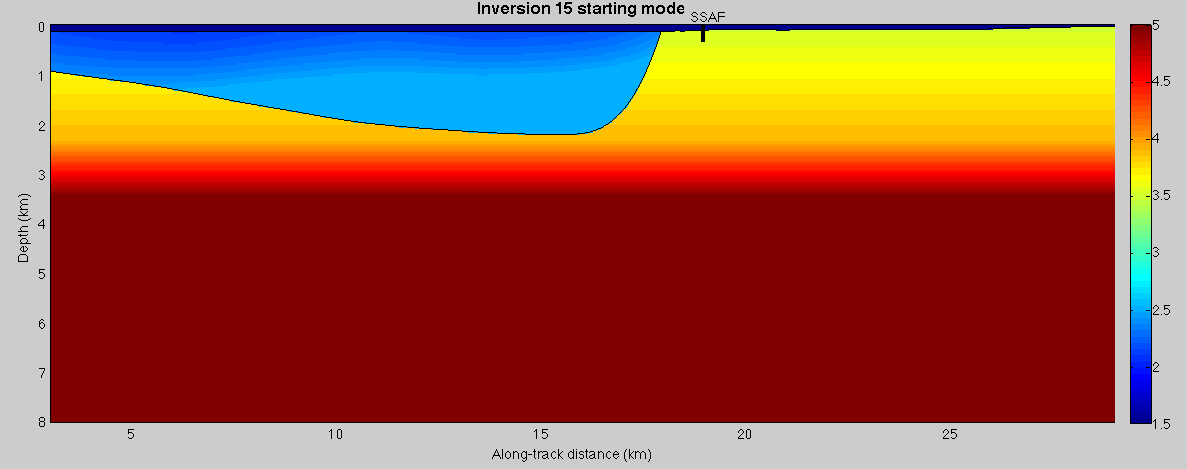
\includegraphics[scale=0.4,keepaspectratio=true]{figs/inv15_0.png}
\caption{Inversion 15 starting model.}
\label{fig:inv15start}
\end{figure}

\clearpage{}

\subexperiment{Raytracing and Inversion Output}
Output found in \autoref{tab:r15} and \autoref{tab:i15}.

%Raytracing Output, INversion 15
\begin{table}[!ht]
\label{tab:r15}
\raggedleft
\begin{tabular}{c l l l l l}
\toprule
\textbf{Raytr, It = } & \textbf{tmean} & \textbf{trms} & \textbf{chi sq} & \textbf{chi r} & \textbf{meanErr} \\
\toprule
It0 & -0.0529 & 0.1197 & 77.0745 & 52.4152 & 0.0241\\
It1 & -0.0222 & 0.1102 & 52.0758 & 47.1082 & 0.0241\\
It2 & -0.0055 & 0.0948 & 29.0273 & 28.6880 & 0.0241\\
It3 & -0.0134 & 0.0696 & 17.7654 & 16.8745 & 0.0241\\
It4 & -0.0135 & 0.0586 & 11.9874 & 11.4367 & 0.0241\\
It5 & -0.0111 & 0.0494 & 7.6122 & 7.5095 & 0.0241\\
It6 & -0.0098 & 0.0456 & 5.6006 & 5.6730 & 0.0241\\
It7 & -0.0105 & 0.0420 & 4.3647 & 4.4582 & 0.0241\\
\bottomrule\\
\end{tabular}
\caption{Inversion 15: Raytracing outputs.}
\end{table}

%Inversion Output, Inversion 15
%INv it 
\begin{table}[!ht]
\label{tab:i15}
\raggedleft
\begin{tabular}{c l l l}
\toprule
\textbf{Inv, It = } & \textbf{set chi sq =} & \textbf{out chi sq =} & \textbf{Penalty} \\
\toprule
It0 & 50 & 50.182 & 144875.5\\
It1 & 30 & 29.006 & 149535.8\\
It2 & 17 & 17.770 & 152034.2\\
It3 & 11 & 11.190 & 153989.8\\
It4 & 7 & 7.1052 & 159624.0\\
It5 & 5 & 5.2451 & 154047.7\\
It6 & 4 & 4.0112 & 153415.7\\
It7 & 3 & & \\
\bottomrule\\
\end{tabular}
\caption{Inversion 15: Inversion outputs.}
\end{table}



 
\end{addmargin}

%----------------------------------------------------------------------------------------
%	BIBLIOGRAPHY
%----------------------------------------------------------------------------------------

\begin{thebibliography}{9}

\bibitem{lamport94}
Leslie Lamport,
\emph{\LaTeX: A Document Preparation System}.
Addison Wesley, Massachusetts,
2nd Edition,
1994.

\end{thebibliography}

%----------------------------------------------------------------------------------------

\end{document}